\documentclass[a4paper, oneside, 12pt]{article}

\usepackage{../custom}

\title{Rapport 2}
\author{Groupe 1225}
\date{\today}

\begin{document}

\maketitle


\section{Calculs énergétiques}

Pour réaliser nos calculs, il est nécessaire de prendre 
en compte la variation possible de 
deux facteurs: $m$ la capacité du plant(en tonnes par jour) 
et $T$ la température à la sortie du
réacteur de reformage à la vapeur de méthane.
Nous obtiendrons donc des formules où ces variables sont des paramètres.

La première réaction analysée est la suivante:

\begin{equation*}
	\ce{CH4 + H2O <-> CO + 3H2}
\end{equation*}

Afin de connaître l'énergie demandée par cette réaction,
il nous faut trouver son avancement. Celle-ci n'est en effet pas complète.
Pour ce faire, nous devons commencer par obtenir la constante $K$ 
de la réaction. Or, elle peut être donnée par la relation:

\begin{equation}
	\ln{(K(T))} = \ln{(K(298.15))} - 
	\frac{\Delta H^{\circ}}{R}(\frac{1}{T} - \frac{1}{298.15})
\end{equation}

L'enthalpie de la réaction à une température est égale 
à la différence pondérée des enthalpies de formation:

\begin{equation}
	\Delta_{reac} H^{\circ} (T)= \Delta_{form,\ce{CO}} H^{\circ}(T)
	+\Delta_{form, \ce{H2}} H^{\circ} (T) - \Delta_{form, \ce{CH4}} H^{\circ} (T) 
	-\Delta_{form, \ce{H2O}} H^{\circ} (T)
\end{equation}

La différence d'enthalpie de formation d'une molécule entre deux 
températures est égale à l'intégrale de sa capacité calorifique 
(à pression fixe) entre ces deux températures.
On utilise donc cette formule en partant de la  température 
standard: $\Delta_{form}H°(T)= \Delta_{form}H°(298.15)+\int_298.15^T Cp(T) \, \mathrm dT$ et pouvons 
remettre notre équation sous la forme suivante:

\begin{equation}
	\Delta_{réac}H°(T)=\Delta_{réac}H°(298.15)+\sum_i \int_{298.15}^T \nu_i Cp_i(T) \, \mathrm dT
\end{equation}

Nous utilisons alors l'approxi_{1}mation suivante pour les différents $C_P$\footnote{http://www.edu.upmc.fr/
chimie/lc101-202-301/communs/public/capcalo.htm}, 
chacun étant sous la forme $a+bT+cT^2$:

\begin{tabular}{|l|c|c|r|}
  \hline
  Gaz & $a$ & $b\e{3}$ & $c\e{6}$ \\
  \hline
  \ce{CH4} & 14,23 & 75,3 & -18,00\\
  \ce{H2O} & 30,13 & 10,46 & 0 \\
  \ce{CO} & 27,62 & 5,02 & 0\\
  \ce{H2} & 29,30 & -0,84 & 2,09\\
  \hline
\end{tabular}

On a alors:
\begin{equation}
	\sum_i \int_298.15^T \nu_i Cp_i(T) \, \mathrm dT=\int_{298.15}^T 71.16-8.326 10^{-2}T+2.427 10^{-5}T^2 \, \mathrm dT
\end{equation}
Une fois l'expression intégrée, on peut simplifier dans l'équation pour trouver l'enthalpie de réaction en 
fonction de la température:

\begin{equation}
	\Delta_{réac}H°(T)=188441.8653+71.16T-4.163 10^-2 T^2 + 8.09 10^-6 T^3
\end{equation}

Maintenant que l'on dispose de cela, il ne nous faut plus qu'une valeur de K à une certaine température 
pour l'obtenir comme une fonction de T. Pour trouver cette valeur particulière, on utilise la 
formule $K(T)=exp(-\frac{\DeltaG°(T)}{RT})$ à la température standard. On trouve facilement $\DeltaG°$ grâce 
aux valeurs des énergies libres de formation (obtenues dans un livre de référence\footnote{Chimie Physique de 
Atkins, DE BOECK} dont on fait la différence pondérée. Le résultat est: $K(298.15)=1.2597*10^-25$.\\
Nous pouvons enfin injecter ces résultats dans notre équation de départ:
\begin{equation}
	ln(K(T))=ln(K(298.15))-\frac{\DeltaH°(T)}{R}(\frac{1}{T}-\frac{1}{298.15})
\end{equation}

Et en simplifiant (attention, le grand nombre de simplification influe sur la précision!):

\begin{equation}
	K(T)=exp(\frac{-22664.245}{T}+10.128+0.0337T+1.5797 10^{-5}T^2+3.263 10^{-9}T^3)
\end{equation}

Faisant exactement de la même manière, on peut obtenir la constante K de la deuxi_{1}ème équation. Tous 
les détails calculatoires sont en annexe sous la forme de code matlab.

\section{Bilan de matière}

Nous cherchons le débit des différents réactifs qu'il faut introduire en fonction de celui de $NH_3$, 
variable, que l'on note $m$[tonnes/jour].

Disposant de cette donnée, on trouve directement le nombre de moles qui y correspond ainsi que 
celles de $H_2$ ($\frac{3m}{34}$) et de $N-2$ ($\frac{m}{34}$) nécessaires  pour cette quantité dans la réaction finale:

\begin{equation*}
	\ce{3H2 + N2 -> 2NH3}
\end{equation*}

Puisque $N_2$ provient de l'apport d'air et que nous connaissons la composition molaire 
de ce dernier (78\% d'\ce{N2}, 21\% d'\ce{O2} et 1\% d'\ce{Ar}), 
on trouve aisément les débit d'air, d'$O_2$ et d'Ar correspondant:

\begin{equation}
	n_{air}/jour=\frac{1}{0.78} n_{N_2}/jour <=> \frac{25 m}{663}
\end{equation}

\begin{equation}
	n_{O_2}/jour=0.21 n_{air}/jour <=> \frac{7 m}{884}
\end{equation}

\begin{equation}
	n_{Ar}/jour=0.01 n_{air}/jour <=> \frac{m}{2652}
\end{equation}

On trouve ensuite les débits molaires au reformage secondaire:
\begin{equation*}
	\ce{2CH4 + O2 -> 2CO + 4H2}
\end{equation*}

\begin{equation}
	n_{CH4}/jour=2 n_{N_2}/jour <=> \frac{7 m}{442}
\end{equation}

\begin{equation}
	n_{CO}/jour=n_{CH_4}/jour
\end{equation}

\begin{equation}
	n_{H_2}/jour <=> \frac{9m}{221}
\end{equation}

Et enfin dans la réaction du Water-Gas-Shift:

\begin{equation*}
	\ce{CO + H2O -> CO2 + H2}
\end{equation*}

\begin{equation}
	n_{CO}/jour=n_{{CH_4}_{secondaire}}+n_{{CH_4}_{primaire}}
\end{equation}

\begin{equation}
	n_{CO_2}/jour=n_{CO}/jour
\end{equation}

A présent, intéressons nous à l'avancement des réactions dans le réacteur primaire. Pour la première réaction, 
à l'équilibre, on a une quantité suivante de réactifs pour un certain \xi_{1}:
	\begin{equation}
	\ce{CH4 + H2O <-> CO + 3H2}
	\end{equation}
	\\
\begin{tabular}{|l|c|c|c|r|}
  \hline
  \ce{CH4} & \ce{H2O} & \ce{CO} & \ce{H2} & n_gaz \\
  \hline
  n_{CH_4} & n_{H_2O} & 0 & 0 & n_{CH_4} + n{H_2O}\\
  n_{CH_4}-\xi_{1} & n_{H_2O}-\xi_{1} & \xi_{1} & $3 \xi_{1}$ & n_{CH_4} + n_{H_2O} + $2 \xi_{1}$\\
  \hline
\end{tabular}
\\
Pour la deuxième équation, avec un certain \xi_{2}:\\
	\begin{equation}
	\ce{CO + H2O <-> CO2 + H2}
	\end{equation}
	\\
\begin{tabular}{|l|c|c|c|r|}
  \hline
  \ce{CO} & \ce{H2O} & \ce{CO2} & \ce{H2} & n_gaz \\
  \hline
   \xi_{1} & n_\ce{H_2O}-\xi_{1} & 0 & $3\xi_{1}$ & n_{H_2O}+$3\xi_{1}$\\
   \xi_{1}-\xi_{2} & n_\ce{H_2O}-\xi_{1}-\xi_{2} & \xi_{2} & $3\xi_{1} +\xi_{2}$ & n_{H_2O}+$3\xi_{1}$\\
  \hline
\end{tabular}
\\
Grâce à cela, on peut obtenir une expression pour les constantes d'équilibres K_1 et K_2:

$$K_1=\frac{{p_{tot}}^2}{{p_0}^2} \frac{1}{(n_\ce{CH4}+n_\ce{H2O}+2\xi_{1})^2} \frac{(\xi_{1}-\xi_{2})(3\xi_{1}+\xi_{2})^{-3}}{(n_\ce{CH4}-\xi_{1})(n_\ce{H2O}-\xi_{1}-\xi_{2})}$$
$$K_2=\frac{\xi_{2} (3\xi_{1}+\xi_{2}}{(\xi_{1}-\xi_{2})(n_\ce{H2O}-\xi_{1}-\xi_{2})}$$

\begin{equation}
K_1=\frac{{p_{tot}}^2}{{p_0}^2} \frac{1}{(n_\ce{CH4}+n_\ce{H2O}+2\xi)^2} \frac{(\xi-\eta)(3\xi+\eta)^{-3}}{(n_\ce{CH4}-\xi)(n_\ce{H2O}-\xi-\eta)}
\end{equation}
\begin{equation}
K_2=\frac{\eta (3\xi+\eta}{(\xi-\eta)(n_\ce{H2O}-\xi-\eta)}
\end{equation}

Ce que l'on peut égaler aux valeurs des constantes trouvées dans la section précédente.

De plus, nous pouvons égaler ce qui sort du réacteur primaire à ce qui rentre dans le réacteur secondaire 
(trouvé précédemment):
\begin{equation}
n_\ce{CH4}-\xi_1=\frac{7m_\ce{NH3}}{442}
\end{equation}

\begin{equation}
3\xi_1+\xi_2=\frac{9m_\ce{NH3}}{221}
\end{equation}

On obtient donc finalement un système de quatre équations à 4 inconnues - où 2 d'entre elles ne sont autres que les débits 
d'\ce{H2O} et de \ce{CH4} -, que nous pouvons résoudre sur Matlab pour plus de facilité (voir annexe). 
Comme prévu, ces quantités dépendent de T et de la masse d'ammoniac voulue à la sortie.

\section{Fonctionnement de l'outil de calcul}

L'outil de calcul a été réalisé en matlab et prends en considération deux variables : la température du 
réacteur primaire (en K) et la quantité d'ammoniac (en tonnes) que l'on souhaite produire en 24h. 
\\

Nous commençons tout d'abord par calculer les enthalpies (incl. Gibbs) et entropies des réactions du réacteur 
primaire (vaporeformage). Nous calculons ensuite les constantes d'équilibres pour les deux réactions. 
Avec les hypothèses posées sur les réactions (toutes sont complètes exceptées celles s'effectuant dans le réacteur primaire),
et avec la masse désirée de \ce{NH3}, nous calculons les masses nécessaires de \ce{H2}, \ce{N2}. Puisque l'azote est fourni
par l'air, nous déterminons la masse de \ce{O2} fournie (ainsi que la masse de \ce{Ar}, mais l'argon est un gaz noble et 
n'intervient pas dans la réaction). 

Avec les hypothèses et la masse de \ce{O2}, nous déterminons la quantité de \ce{CH4} 
utilisé dans le réacteur secondaire et donc la production de \ce{H2} dans ce réacteur. Nous savons désormais 
déterminer la quantité de \ce{H2} à produire dans le réacteur primaire, et grâce à la constante d'équilibre déterminée 
plus tôt, nous pouvons déterminer la quantité de \ce{CH4} nécessaire pour les deux réactions. L'outil nous permet également
de calculer la quantité minimum de \ce{H2O} à fournir pour que toutes les équations se passent comme prévu. 
\\

Il est à noter que l'outil nous fourni des valeurs en tonnes par jour.

\section{Tubes}
Nous recherchons le nombre de tubes nécaissaire à l'acheminement du méthane et de l'eau dans le reformateur primaire.\\
\\
Soit $x$ le nombre de tubes, nous avons l'équation suivante :
\[
V'_{(m^3/s)} = A_{(m^2)}. c'_{(m/s)} .x
\]
Avec $V'$ le débit; $A$ la section d'un tuyau et $c'$ la vitesse superficielle à l'entrée du réacteur.\\
\\
Le volume peut être calculé grace à la loi des gaz parfaits;
\[
V=\frac{nRT}{P}
\]

Si l'on concidère notre calcul en un espace de temps d'1 seconde. La simplification des deux formules ci-dessus nous amène à
\[
x=\frac{nRT}{AcP}
\]
Ou la seule inconnue est les nombre de môles de produit rentrant, c'est a dire de $CH_{4}$ et de $H_{2}O$. Ce que nosu avons pu déterminer grace au programme MATLAB sachant que 1500 T d'ammoniac était demandée à la sortie.\\
\\
$n_{CH_{4}}= 7,56_{kg} / 0,016_{kg/mole} = 472,18 moles$\\
$n_{H_{2}O}= 18,94_{kg/s}/ 0,016_{kg/mole} = 1052,22 moles$\\

Grâce aux autres valeurs données dans l'énoncé nous pouvons calculer le nombre de tubes nécessaire 


\[
x=\frac{(n_{CH_{4}}+n_{H_{2}O})8,314.1080}{\pi(0,05^2).2.(31.10^5)}=281,1
\]

Il faut donc 282 tuyaux pour assurer l'approvionnnement des composés dans le reformateur primaire.

\begin{figure}[htp]
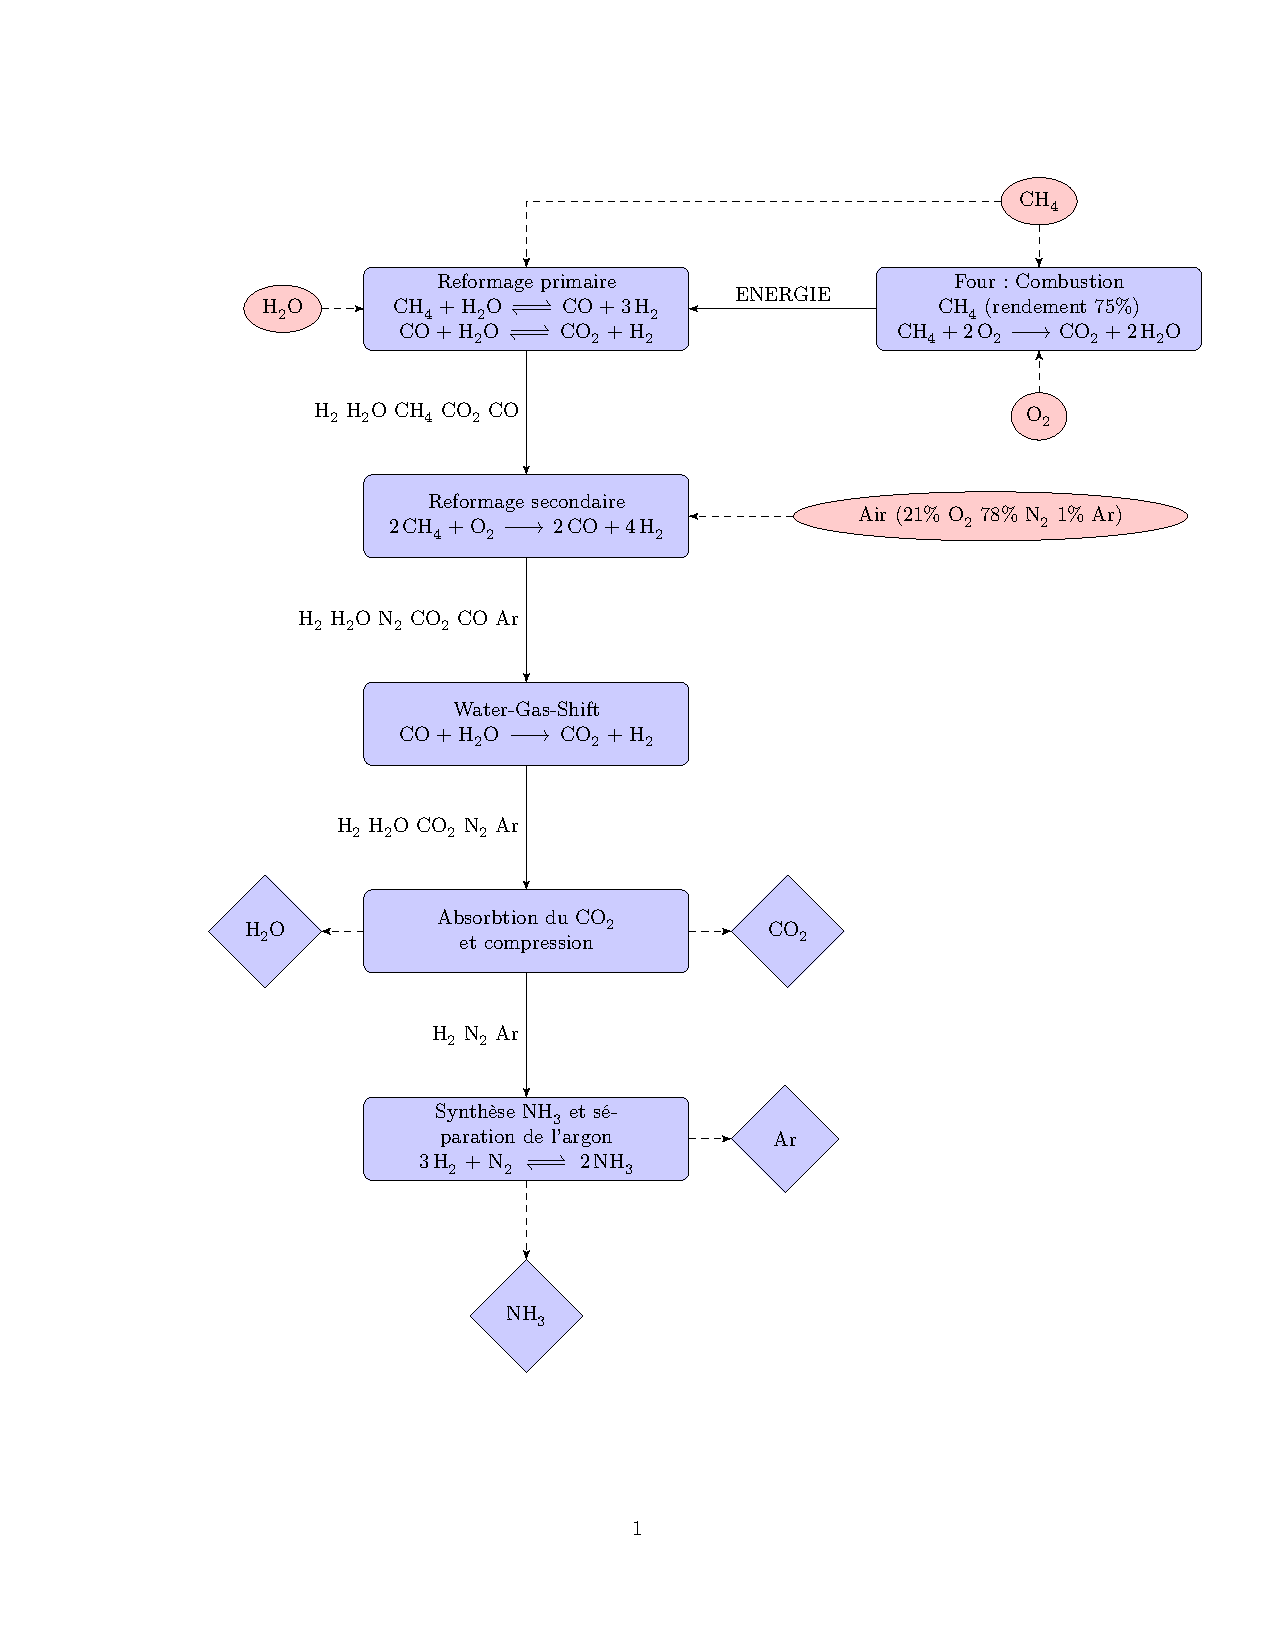
\includegraphics[scale=0.82]{flow_sheet.pdf}

	%\begin{tikzpicture}
[node distance = 7em]

\tikzstyle{decision} = [diamond, draw, fill=blue!20, 
    text width=4.5em, text badly centered, node distance=3cm, inner sep=0pt]
\tikzstyle{block} = [rectangle, draw, fill=blue!20, 
    text width=15em, text centered, rounded corners, minimum height=4em]
\tikzstyle{line} = [draw, -latex']
\tikzstyle{cloud} = [draw, ellipse,fill=red!20, node distance=3cm,
    minimum height=2em]
    
\node [block] (primaire) {Reformage primaire (T)\\
\ce{CH4 + H2O <=> CO + 3H2} \\
\ce{CO + H2O <=> CO2 + H2}};
\node [cloud, left = 2em of primaire] (H2O) {\ce{H2O}};
\node [block, right = 2em of primaire] (four) {Four: Combustion \ce{CH4} (rendement $75\%$) ($\simeq 1300K$)\\
\ce{CH4 + 2O2 -> CO2 + 2H2O}};
	\node [cloud, below = 2em of four] (O2) {\ce{O2}};
	\node [cloud, above = 2em of four] (CH4) {\ce{CH4}};
\node [block, below of=primaire] (secondaire) {Reformage secondaire ($\simeq 1200K$)\\
\ce{2CH4 + O2 -> 2CO + 4H2}};
	\node [cloud, right = 1em of secondaire] (air) {Air ($21\% \ce{O2} 78\% \ce{N2} 1\% \ce{Ar}$)};
	\node [block, below of=secondaire] (wgs) {Water-Gas-Shift ($\simeq 500-700K$)
\ce{CO + H2O -> CO2 + H2}};
\node [block, below of=wgs] (abso) {Absorbtion du \ce{CO2} et compression};
	\node [decision, right = 2em of abso] (CO22) {\ce{CO2}};
	\node [decision, left = 2em of abso] (H2O2) {\ce{H2O}};
	\node [block, below of=abso] (synthese) {Synthèse \ce{NH3} et séparation de l'argon \\
(Sortie réacteur: 270bar, 750K) \\
\ce{3H2 + N2 <=> 2NH3}};
\node [decision, below of=synthese] (NH3) {\ce{NH3}};
\node [decision, right = 2em of synthese] (argon) {\ce{Ar}};


	\path [line] (primaire) -- node[anchor = east] {\ce{H2} \ce{CH4} \ce{CO2} \ce{CO} \ce{H2O}}(secondaire);
	\path [line] (four) -- node[anchor = south] {\textbf{E}}(primaire);
    \path [line,dashed] (CH4) -- (four);
    \path [line,dashed] (CH4) -| (primaire);
    \path [line,dashed] (O2) -- (four);
    \path [line] (secondaire) -- node[anchor = east] {\ce{H2} \ce{N2} \ce{CO2} \ce{CO} \ce{Ar} \ce{H2O}}(wgs);
    \path [line] (wgs) -- node[anchor = east] {\ce{H2} \ce{H2O} \ce{CO2} \ce{N2} \ce{Ar}}(abso);
    \path [line] (abso) -- node[anchor = east] {\ce{H2} \ce{N2} \ce{Ar}}(synthese);
\path [line,dashed] (synthese) -- (NH3);
\path [line,dashed] (synthese) -- (argon);
\path [line,dashed] (air) -- (secondaire);
\path [line,dashed] (H2O) -- (primaire);
\path [line,dashed] (abso) -- (CO22);
\path [line,dashed] (abso) -- (H2O2);

\end{tikzpicture}


	\caption{Flow-sheet}
\end{figure}


\end{document}
